\section{実装}
本章では『わかるらんど』の実装について述べる。

\subsection{クライアント}
クライアントはHTML/CSS/JavaScriptで実装しており、通常のブラウザ上で動作するWebアプリケーションとして動作する.

\subsection{サーバ}
サーバは並列計算プリミティブLindaをWebサーバ上に実装したlinda-server\footnote{https://github.com/node-linda/linda}を用いて実装している。

\subsubsection{Linda}
Lindaは、複数のプロセスで共有される空間を用いてプロセス間通信や
データ共有をサポートする分散並列処理を行うためのモデルである。
プロセスが共有する空間はタプル空間 (Tuple Space) と呼ばれ、
タプル空間内のデータ (Tuple) を使って通信やデータ共有を行う (図\ref{linda})。
このように Linda のモデルはきわめて単純であるが、
各クライアントやデバイス間で直接送信をする処理を記述する必要がなく,
柔軟で強力なプロセス間通信を容易に記述することができる。

\begin{figure}[h]
\centering
\fbox{
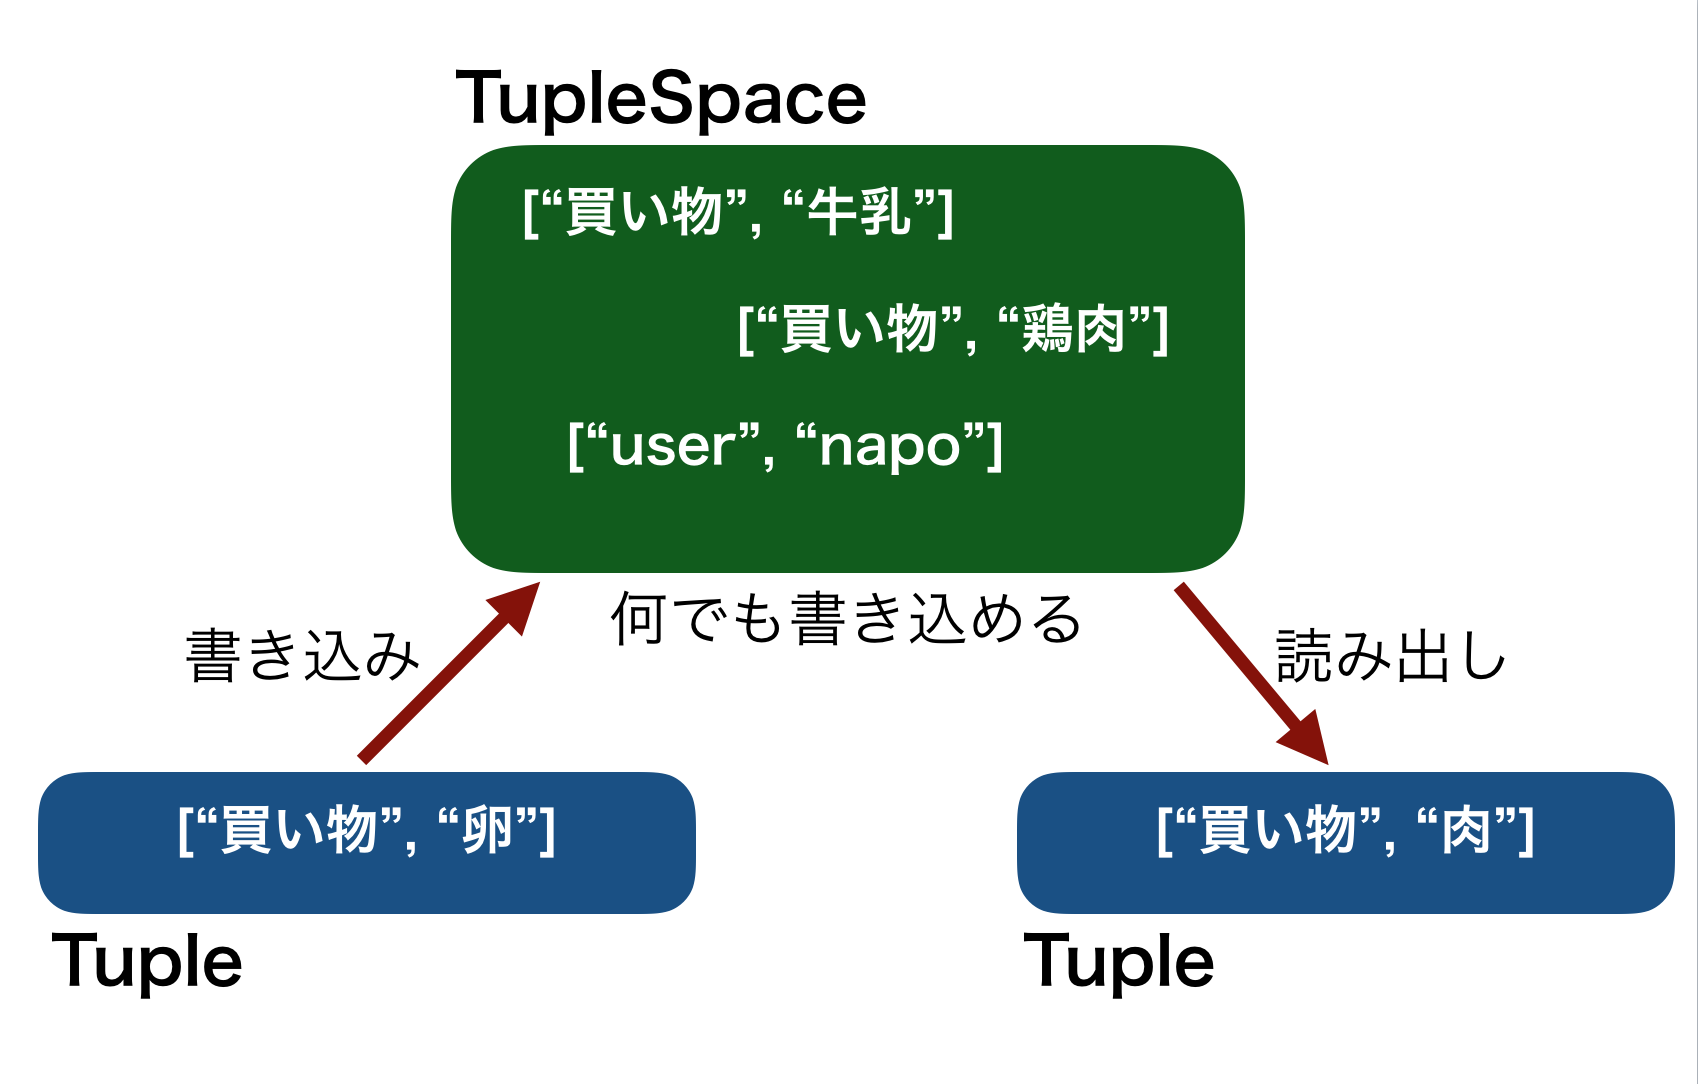
\includegraphics[width=7cm]{images/linda.png}
}
\caption{Linda}
\label{button}
\end{figure}

\subsubsection{linda-server}
linda-serverは、Node.js\footnote{https://nodejs.org}のWebSocketライブラリSocket.IO\footnote{http://socket.io}上に実装されたLindaシステムである。
linda-serverは、橋本翔氏\footnote{http://shokai.org}が開発したオープンソースソフトウェアである。
linda-serverは、\url{write, read, watch, take}の4つの基本操作によってプロセス間通信を行う。

write

新しいデータオブジェクト(タプル)を生成し共有空間(タプルスペース)に書き込む。
例えば、

ts.write(\{type: "sensor", name: "明るさ", value: 123\});

とすると、タプルスペースに、

{type: "sensor", name: "明るさ", value: 123}

というオブジェクトが書き込まれる。


read

指定した形式に部分一致するタプルがタプルスペースにあるかどうか調べて1つ読み出す。
たとえば、タプルスペースに、

{type: "sensor", name: "温度", value: 20}

{type: "sensor", name: "明るさ", value: 123}

{type: "sensor", name: "明るさ", value: 400}

が存在する状態で、

ts.read({type: "sensor", name: "明るさ"})

を実行すると、

{type: "sensor", name: "明るさ", value: 400}

が読み出される。

\url{read}はコールバックなので、一致するものが無い場合は一致するタプルが書き込まれるまで待つ。